\documentclass[9pt]{article}
\usepackage[margin=0.5in]{geometry}
\usepackage{graphicx}
\usepackage{amsmath}
\usepackage{listings}
\usepackage{xcolor}
\usepackage{hyperref}
\usepackage{subcaption}
\usepackage{float}
\usepackage{enumitem}
\usepackage{multicol}
% Remove indentation and minimize spacing for all itemize lists
\setlist[itemize]{
    noitemsep,           % No space between items
    topsep=0pt,          % No space before/after list
    partopsep=0pt,       % No extra paragraph space
    leftmargin=0pt,      % No left indentation
    itemindent=1em,      % Indent for the bullet itself
    labelsep=0.5em       % Space between bullet and text
}

% Code listing settings
\lstset{
    language=Python,
    basicstyle=\ttfamily \scriptsize,
    keywordstyle=\color{blue},
    commentstyle=\color{gray},
    stringstyle=\color{red},
    numberstyle=\tiny\color{gray},
    stepnumber=1,
    numbersep=5pt,
    backgroundcolor=\color{white},
    showspaces=false,
    showstringspaces=false,
    showtabs=false,
    frame=single,
    tabsize=2,
    captionpos=b,
    breaklines=true,
    breakatwhitespace=false,
    escapeinside={\%*}{*)},
    columns=flexible,
    morekeywords={
        np, cv, array, linspace, arange, reshape, dtype,
        zeros, ones, eye, mean, median, std, var,
        sum, max, min, clip, concatenate, hstack, vstack,
        imread, imshow, imwrite, cvtColor, COLOR_BGR2GRAY,
        GaussianBlur, filter2D, Sobel, Laplacian,
        bitwise_and, threshold, inRange, findContours,
        moments, boundingRect, rectangle, circle,
        waitKey, destroyAllWindows, LUT, calcHist, power, merge, astype,
        split, transformation
    }
}

\title{\textbf{EN3160 Assignment 2: Fitting and Alignment}}
\author{
    Balasooriya B.A.P.I \\
    \texttt{220054N} \\
    \href{https://github.com/PankajaBalasooriya/EN3160_Image_Processing_and_Machine_Vision.git}{%
        
\includegraphics[width=0.02\textwidth]{resources/github-mark.png}\hspace{0.5em}%
        \texttt{PankajaBalasooriya/EN3160\_Image\_Processing\_and\_Machine\_Vision}%
    }\\[0.05cm]
    \href{https://github.com/PankajaBalasooriya/EN3160_Image_Processing_and_Machine_Vision/blob/main/Assignments/Assignment1_PointOperationsAndSpatialFiltering/assignment1.ipynb}{%
        
\includegraphics[width=0.02\textwidth]{resources/jupyter-icon.png}\hspace{0.5em}%
        \texttt{View Jupyter Notebook}%
    }
}
\date{}

\begin{document}

\maketitle

% \begin{abstract}
% This report presents solutions to four problems in computer vision: blob detection using Laplacian of Gaussians for circle detection in sunflower images, RANSAC-based line and circle fitting to noisy point sets, homography-based planar warping for flag superimposition, and image stitching using SIFT features and homography estimation.
% \end{abstract}

\section{Blob Detection}
% \subsection{Methodology}
Blob detection was implemented using Laplacian of Gaussians (LoG) across multiple scales. The key steps are,
\begin{itemize}
    \item Implementing LoG
\begin{lstlisting}
def LoG_kernal(sigma):
    half_width = int(ceil(3*sigma))
    width = 2*half_width + 1
    y, x = np.mgrid[-half_width:half_width+1, -half_width:half_width+1]
    r_2 = x**2 + y**2
    # Laplacian of Gaussian formula
    LoG = -1/(np.pi * sigma**4) * (1 - r_2/(2*sigma**2)) * np.exp(-r_2/(2*sigma**2))
    LoG -= LoG.mean()   # making the sum of kernel elements zero
    return LoG
\end{lstlisting}
    \item Scale-space construction using Gaussian kernels with varying $\sigma$ values
\begin{lstlisting}
height, width = normalized_img.shape
scale_space = np.zeros((height, width, n_levels), dtype=np.float32)

for i, sigma in enumerate(sigmas):
    LoG = LoG_kernal(sigma)
    filtered_img = cv.filter2D(normalized_img, -1, LoG)
    # Scale-normalized LoG response of the squared Laplacian response
    scale_space[:, :, i] = (sigma**2) * np.abs(filtered_img)
\end{lstlisting}
    \item Finding the maxima in the scale space using Non-maximum suppression across spatial and scale dimensions
    \begin{itemize}
        \item 2D Non-maximum suppression
\begin{lstlisting}
def nonmax2d(response, neighborhood=3):
    """boolean mask of the local maxima in a neighborhood."""
    if neighborhood % 2 == 0:
        neighborhood += 1
    footprint = np.ones((neighborhood, neighborhood), dtype=bool)
    local_max = ndimage.maximum_filter(response, footprint=footprint, mode='reflect')
    mask = (response == local_max)
    return mask

nms2d_masks = np.zeros_like(scale_space, dtype=bool)
for i in range(n_levels):
    nms2d_masks[:, :, i] = nonmax2d(scale_space[:, :, i], neighborhood=3)

\end{lstlisting}
        \item 3D Non-maximum suppression (across scales)
\begin{lstlisting}
candidates = []
for i in range(n_levels):
    resp = scale_space[:, :, i]
    mask2d = nms2d_masks[:, :, i]
    if i == 0:
        is_scale_max = (resp >= scale_space[:, :, i+1])
    elif i == n_levels - 1:
        is_scale_max = (resp >= scale_space[:, :, i-1])
    else:
        is_scale_max = (resp >= scale_space[:, :, i-1]) & (resp >= scale_space[:, :, i+1])
        
    final_mask = mask2d & is_scale_max
    ys, xs = np.nonzero(final_mask)
    for y, x in zip(ys, xs):
        candidates.append((y, x, i, float(resp[y, x])))
\end{lstlisting}

    \end{itemize}
    \newpage
    \begin{multicols}{2}
        \item Threshold and Ranking
\begin{lstlisting}
threshold = 0.31 
max_blobs = 1000

# filter by threshold and convert scale index to sigma
blobs = []
for (y, x, scale_idx, resp_val) in candidates:
    if resp_val >= threshold:
        sigma = sigmas[scale_idx]
        blobs.append((y, x, sigma, resp_val))

# sort and keep top
blobs.sort(key=lambda b: b[3], reverse=True)
blobs = blobs[:max_blobs]
\end{lstlisting}
\newcolumn
    \item Draw circles around blobs
\begin{lstlisting}
def draw_blobs(img_bgr, blobs, radius_factor=sqrt(2), color=(0,0,255)):
    out = img_bgr.copy()
    for (y, x, sigma, resp) in blobs:
        r = int(round(radius_factor * sigma))
        cv.circle(out, (int(x), int(y)), r, color, 1, lineType=cv.LINE_AA)
    return out
\end{lstlisting}
\textbf{Parameters}\\ 
Scale range $\sigma \in [2.0, 15.0)$, $12$ scales with a scaling factor $k=1.2$
    \end{multicols}
    
\end{itemize}



\subsection{Results}
\begin{multicols}{2}
\begin{figure}[H]
    \centering
    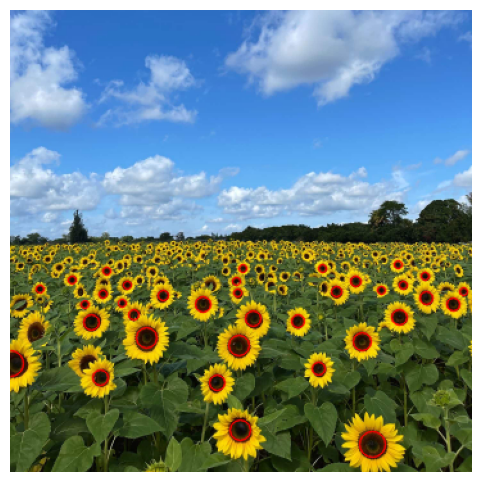
\includegraphics[width=0.9\columnwidth]{resources/sunflowe_blobs.png}
    \caption{Detected circles in sunflower field image}
    \label{fig:sunflowers}
\end{figure}

\subsubsection*{Largest Circles:}

Circle 1: Center $(282.00,	338.00)$, Radius $10.0$, $\sigma$ 7.17\\
Circle 2: Center $(0.00,275.00)$, Radius $10.0$, $\sigma$ 7.17\\
Circle 3: Center $(106.00,255.00)$, Radius $8.00$, $\sigma$ 5.97



\subsection{Discussion}
The LoG detector successfully identifies blob structures at multiple scales. The relationship between $\sigma$ and circle radius follows $r = \sqrt{2}\sigma$.
\end{multicols}

\section{RANSAC Line and Circle Fitting}
\begin{multicols}{2}
\subsection{Line Fitting with RANSAC}
\begin{lstlisting}[caption={RANSAC line fitting}]
def ransac_line(points, n_iter=500, thr=1.2, min_inliers=30):
    N = len(points)
    best_inliers = []
    best_sample = None
    best_model = None
    for i in range(n_iter):
        idx = np.random.choice(N, 2, replace=False)
        p1, p2 = points[idx[0]], points[idx[1]]
        model = fit_line_from_two_points(p1, p2)
        if model is None:
            continue
        a,b,d = model
        errs = line_point_error(a,b,d,points)
        inliers = np.where(errs <= thr)[0]
        if len(inliers) > len(best_inliers):
            best_inliers = inliers
            best_sample = idx
            best_model = model
            
    refined = fit_line_tls(points[best_inliers])
\end{lstlisting}

\textbf{Parameters:}
\begin{itemize}
    \item Iterations: 800
    \item Distance threshold: 1.2
\end{itemize}
After removing line inliers, fit circle to remaining points,
\newcolumn
\subsubsection{Circle Fitting with RANSAC}

\begin{lstlisting}[caption={RANSAC circle fitting}]
def ransac_circle(points, n_iter=1000, thr=1.0, min_inliers=20):
    N = len(points)
    best_inliers = []
    best_model = None
    best_sample = None
    for i in range(n_iter):
        idx = np.random.choice(N, 3, replace=False)
        p1, p2, p3 = points[idx[0]], points[idx[1]], points[idx[2]]
        model = circle_from_3pts(p1, p2, p3)
        if model is None:
            continue
        x0, y0, r0 = model
        errs = circle_radial_error(x0, y0, r0, points)
        inliers = np.where(errs <= thr)[0]

        if len(inliers) > len(best_inliers):
            best_inliers = inliers
            best_model = (x0, y0, r0)
            best_sample = idx
\end{lstlisting}

\begin{itemize}
    \item Sample size: 3 points
    \item Error metric: Radial distance
    \item Threshold: 1.0
\end{itemize}
\end{multicols}

\begin{multicols}{2}
\subsection{Results}
\begin{figure}[H]
    \centering
    \includegraphics[width=\columnwidth]{resources/ransac.png}
    \caption{RANSAC fitting results showing point set, inliers, and estimated models}
    \label{fig:ransac}
\end{figure}

\textbf{Estimated Parameters}\\[4pt]
\textbf{Line:}\\
Initial model: $a = 0.7246,\; b = 0.6892,\; d = 1.2435$\\
Refined model: $a = -0.7192,\; b = -0.6948,\; d = -1.3423$\\
Line inliers: 55 points\\[8pt]

\textbf{Circle:}\\
Initial model: $x_0 = 1.9791,\; y_0 = 3.0529,\; r = 10.1662$\\
Refined model: $x_0 = 1.9706,\; y_0 = 3.2490,\; r = 10.0412$\\
Final refined (from mapped inliers): $x_0 = 1.9706,\; y_0 = 3.2490,\; r = 10.0412$\\
Circle inliers: 36 points\\



\\
\textbf{Fitting circle first}\\ If the circle is fitted first, it might accidentally pick 3 points that belong to the line, producing a large-radius circle or a wrong center, because some line points can be consistent with a circle hypothesis, especially if they are near parts of the circle or if there is noise. This can produce a spurious consensus set that includes many line points.

\end{multicols}



\section{Homography and Planar Warping}

\subsection{Methodology}
Implemented homography-based warping for flag superimposition:
\begin{enumerate}
    \item Select 4 correspondence points on target plane
    \item Compute $3 \times 3$ homography matrix $\mathbf{H}$
    \item Warp flag image using perspective transformation
    \item Blend warped flag onto target image
\end{enumerate}

The homography satisfies: $\mathbf{x}' = \mathbf{H}\mathbf{x}$ where $\mathbf{x}$ and $\mathbf{x}'$ are homogeneous coordinates.

\begin{lstlisting}[caption={Homography computation}]
def compute_homography(src_pts, dst_pts):
    # Build matrix A from correspondences
    # Solve Ah = 0 using SVD
    # Reshape to 3x3 matrix
    return H
\end{lstlisting}

\subsection{Results}
\begin{figure}[H]
    \centering
    \begin{subfigure}{0.48\columnwidth}
        \includegraphics[width=\textwidth]{example1.png}
        \caption{Example 1}
    \end{subfigure}
    \begin{subfigure}{0.48\columnwidth}
        \includegraphics[width=\textwidth]{example2.png}
        \caption{Example 2}
    \end{subfigure}
    \caption{Flag warping results on different architectural images}
    \label{fig:homography}
\end{figure}

\subsection{Image Selection Rationale}
Selected images with clear planar surfaces (walls, boards) for accurate homography estimation. The planar assumption is critical for correct perspective transformation.

\section{Image Stitching with SIFT}

\subsection{SIFT Feature Matching}
\begin{itemize}
    \item Detected SIFT keypoints and descriptors
    \item Matched features using nearest neighbor ratio test
    \item Filtered matches with ratio threshold (typically 0.7-0.8)
\end{itemize}

\subsection{Homography Estimation}
Implemented RANSAC-based homography estimation:

\begin{lstlisting}[caption={RANSAC homography}]
def ransac_homography(matches, iterations, threshold):
    for i in range(iterations):
        # Sample 4 correspondences
        # Compute homography
        # Count inliers using reprojection error
        # Update best model
    return best_H, inliers
\end{lstlisting}

\subsection{Results}
\begin{figure}[H]
    \centering
    \includegraphics[width=\columnwidth]{stitched_result.png}
    \caption{Stitched panorama of Graffiti images}
    \label{fig:stitch}
\end{figure}

\textbf{Comparison with Ground Truth:}
\begin{itemize}
    \item Estimated $\mathbf{H}$: [matrix values]
    \item Ground truth $\mathbf{H}$: [matrix values]
    \item Frobenius norm error: $\|\mathbf{H}_{est} - \mathbf{H}_{gt}\|_F = \ldots$
\end{itemize}

Number of SIFT matches: XXX, Inliers: YYY

\subsection{Discussion}
The RANSAC approach effectively handles outliers in feature matching. The estimated homography closely matches ground truth, validating the implementation. Minor discrepancies arise from feature localization errors.

% \section{Conclusion}
% Successfully implemented blob detection, RANSAC-based model fitting, homography estimation, and image stitching. Key insights include the importance of appropriate threshold selection in RANSAC and the robustness of SIFT features for wide-baseline matching.

% \section*{GitHub Repository}
% Complete code and commit history available at: \\
% \url{https://github.com/yourusername/EN3160-Assignment2}

\end{document}